\documentclass[11pt,journal,onecolumn,draftclsnofoot]{IEEEtran}

\IEEEoverridecommandlockouts
\usepackage{newtxtext,newtxmath}
\usepackage{amsmath,amssymb}
\usepackage{graphicx}
\usepackage{booktabs}
\usepackage{array}
\usepackage{enumitem}
\usepackage{float}
\usepackage{tikz}
\usetikzlibrary{positioning,arrows.meta,shapes.geometric}
\usepackage{algorithm}
\usepackage{algpseudocode}
\usepackage{cite}
\usepackage{hyperref}
\hypersetup{
    colorlinks=true,
    linkcolor=black,
    citecolor=black,
    urlcolor=black
}

\setlist[itemize]{leftmargin=1.4em}
\setlist[enumerate]{leftmargin=1.6em}

\title{Learning Topology-Aware Cooperative Caching Policies for IoT Edge Networks}
\author{Abdullah Al Mujahid, Asir Abrar, and Monideepa Kundu Sinthi}

\begin{document}

\maketitle

\begin{abstract}
Edge caching reduces delay and backhaul load by placing content near users, but IoT edge networks are difficult caching environments because user mobility changes both demand and the effective cooperation topology among edge nodes. We study topology-aware cooperative caching in a graph-based IoT edge system where access points act as edge caches and mobility-induced handoffs define weighted inter-node relationships. We formulate cache placement as a stochastic online optimization problem that jointly considers access cost, replication overhead, topology-aware redundancy, relocation cost, and optimization overhead under random topology perturbations. To solve the problem, we propose Adaptive TACC, a reproducible pipeline that combines topology-aware greedy placement, transition-aware DQN refinement, and a cost-aware validation selector that changes the deployed placement only when the expected benefit justifies cache rewriting. Because the Dartmouth campus WLAN trace is publicly described but not directly downloadable through legacy unauthenticated URLs at the time of this study, we record the official dataset access path and use a deterministic trace-compatible mobility generator for reproducible evaluation. Experiments over a 20-node mobility graph, 48-object catalog, and repeated perturbation samples show that DQN is useful when it is used as an online local-refinement operator rather than as a fixed alternative placement. Adaptive TACC selects online DQN refinement in all four tested perturbation windows, improving objective from 2.633 to 2.209 in the stable window and from 5.252 to 3.555 at \(p=0.15\), while explicitly reporting the relocation cost of each cache update.

\end{abstract}

\textbf{Keywords:} IoT edge caching, cooperative caching, topology-aware optimization, mobility graph, Zipf demand, deep reinforcement learning, DQN.

\section{Introduction}

Edge caching is a fundamental mechanism for reducing content-access latency, lowering backhaul traffic, and improving service availability in IoT and edge-computing systems. By storing popular or delay-sensitive content at access points (APs), gateways, roadside units, or small-cell base stations, an edge network can serve requests close to where they originate rather than repeatedly contacting a remote origin. This idea has become increasingly important as edge systems support augmented reality, autonomous mobility, real-time sensing, local analytics, and collaborative edge intelligence workloads \cite{Satyanarayanan2017Edge,Chiang2016Fog,Bastug2014,Mao2017MEC,bai2025collaborative}. The benefit of caching, however, depends not only on which objects are popular, but also on where cached objects are placed relative to users, edge nodes, and the network paths that connect them.

Most simple caching rules are not designed for this setting. Local popularity caching optimizes each cache independently and ignores the fact that neighboring nodes may cooperate. Global popularity caching stores the same highly requested objects at many nodes, which can improve the hit rate for a small set of objects but often reduces the distinct content footprint available across the cooperative network. Classical replacement policies such as LRU and LFU are useful online baselines, yet they do not explicitly reason about graph structure, mobility, or cooperation among edge caches \cite{Podlipnig2003,Li2018CachingSurvey}. Cooperative wireless caching and FemtoCaching demonstrate that coordinated helper placement can substantially improve delivery efficiency \cite{Shanmugam2013,Golrezaei2014JSAC}, but static helper assumptions become restrictive when the effective cooperation graph changes with mobility.

Mobility is a central source of structure in IoT edge caching. In a campus WLAN, industrial IoT deployment, smart-city network, or vehicular edge system, users and devices repeatedly associate with different APs or edge nodes. These transitions create a behavioral graph: two APs connected by frequent handoffs are likely to serve overlapping populations, observe related demand, and benefit from coordinated cache placement. Handoff graphs and neighbor graphs have been studied for WLAN mobility modeling and handoff optimization \cite{kim2005mobility_wifi_ap,shin2004neighbor_graphs}. In this work, we use the same kind of mobility-derived structure for cooperative caching. The graph is not a decorative feature; it determines which cached objects are reachable, how expensive cooperative retrieval is, and where duplicate placement is wasteful.

The central research problem is therefore to determine how edge caches should coordinate when the cooperation topology is induced by mobility and may be perturbed. A robust placement must balance several competing terms. Local storage reduces access delay but consumes capacity. Replication can reduce origin misses but may duplicate content at strongly related nodes. Diversity improves the cooperative catalog footprint but may place popular objects farther from their strongest demand. Relocation allows the system to respond to graph changes but creates update overhead. These trade-offs are widely recognized in caching and MEC research, where hit ratio alone is insufficient to characterize operational performance \cite{Paschos2018RoleCaching,Poularakis2014Approx,Wang2017Mobility}.

We formulate topology-aware cooperative caching as a stochastic online graph optimization problem. Edge nodes form a weighted graph whose edge weights are derived from mobility-induced AP handoffs. Content demand is represented by a node-object probability matrix. A binary placement matrix determines which objects are stored at each node subject to cache-capacity constraints. The objective combines expected access cost, replication cost, edge-weighted redundancy, and relocation cost under sampled graph perturbations. Perturbations remove nodes and edges to model temporary AP unavailability, weakened cooperative links, and changing mobility windows. Under this model, the same placement can have different value across graph realizations because reachable cache holders, shortest-path retrieval costs, redundancy relationships, and origin misses all change. Since the controller is online, relocation is measured against the previously deployed placement rather than against an isolated static baseline.

We propose Adaptive TACC, a topology-aware cooperative caching method that combines structured optimization, transition-aware learning-based local refinement, and cost-aware policy selection. The method first constructs strong candidate placements by selecting node-content pairs with high expected marginal objective reduction under perturbation samples and by building diversity-aware alternatives. It then applies a compact DQN refiner to the currently deployed cache state rather than training a neural policy over the full binary placement space from scratch. During inference, a DQN action is accepted only if it improves the measured online objective against the current cache state, which keeps learning conservative and limits harmful relocation. Finally, Adaptive TACC selects among strong candidate placement families using held-out perturbation samples and an optimization-cost penalty. This selector is part of the method because the best cache-quality policy is not always the best operating policy if its marginal gain is too small to justify cache rewriting and computation.

The study makes the following contributions:
\begin{itemize}
    \item We develop a stochastic online topology-aware cooperative caching formulation that integrates mobility-derived graph structure, access cost, replication overhead, redundancy among strongly related nodes, and relocation cost against the previously deployed cache state.
    \item We design Adaptive TACC, a policy architecture that combines topology-aware greedy placement, transition-aware DQN local refinement, and cost-aware validation selection across perturbation regimes.
    \item We construct a reproducible evaluation protocol for AP handoff graphs, Zipf-locality demand, graph perturbation, and multi-metric cache evaluation when mobility traces do not include application-layer content requests.
    \item We compare Adaptive TACC against random placement, local popularity, global popularity, diversified popularity, topology-aware greedy, fixed Greedy+DQN refinement, and online DQN refinement across repeated topology perturbation samples.
    \item We show that the useful role of DQN is transition-aware refinement of the current deployed cache. Fixed Greedy+DQN improves over topology-aware greedy, but online DQN refinement produces the strongest objective in every tested perturbation window because it improves the current cache without requiring an uncontrolled rewrite.
\end{itemize}

The resulting contribution is not a claim that a DQN alone solves cooperative caching. Rather, the result is that mobility-derived topology should shape cache placement, learning should refine the deployed cache state rather than replace it wholesale, and policy selection should account for both cache quality and the operational cost of changing cache contents.

\section{Background and Challenges}

\subsection{IoT Edge Caching}

In an IoT edge network, devices generate requests through nearby infrastructure such as APs, gateways, base stations, or edge servers. If the requested object is cached locally, the request is served with low delay. If not, the node may retrieve the object from a neighboring edge cache or from a remote origin. Cooperative caching improves coverage by letting nodes use nearby caches, but cooperation is not free: retrieving from another node has communication delay, and storing duplicate objects in nearby caches can waste limited storage.

\subsection{Mobility-Induced Topology}

The key modeling choice is the use of mobility as a topology signal. APs that exchange many users through handoffs are not merely physically close; they are behaviorally related. Their users may request similar content, and content missed at one AP may soon be needed at another. Handoff graphs and neighbor graphs have been used in WLAN mobility analysis and handoff optimization \cite{kim2005mobility_wifi_ap,shin2004neighbor_graphs}. We reuse that idea for cooperative caching: mobility-derived edges become the structure over which cache cooperation is evaluated.

\subsection{Why Local Caching Is Insufficient}

Node-local policies such as local popularity caching are scalable and simple, but they ignore the fact that nearby nodes can cooperate. If every AP stores only its own top objects, the system may miss opportunities to diversify neighboring caches. Conversely, if every AP stores the same globally popular objects, local hit rates may improve for the most popular objects, but many requests still go to the origin because the cooperative cache footprint is small. Effective edge caching must balance popularity, diversity, and graph distance.

\subsection{Dynamic Perturbations}

The effective edge graph may change because APs become unavailable, users move differently, or links become less useful. A robust policy should remain useful under perturbed graphs, not only under the nominal graph. However, adapting cache placement has a cost. Rewriting caches too frequently consumes bandwidth and storage operations, and it may be infeasible for resource-constrained edge devices. This motivates an objective with both access efficiency and relocation stability.

\subsection{Partial Observability of Demand}

The Dartmouth campus WLAN trace provides AP association behavior but not content requests. This is common in mobility datasets, where network-level traces do not include application-layer object identities. A research-level caching study must therefore distinguish between real mobility structure and synthetic demand assumptions. In this paper, the mobility topology is trace-compatible, while content demand is generated using a transparent Zipf-locality model.

\subsection{Design Requirements}

The challenges above translate into five design requirements:
\begin{itemize}
    \item \textbf{Topology awareness}: the policy must reason about which nodes can cooperate cheaply.
    \item \textbf{Demand locality}: nodes should be allowed to have different content preferences.
    \item \textbf{Diversity control}: neighboring nodes should not blindly store identical objects.
    \item \textbf{Perturbation robustness}: placements should be evaluated under graph changes.
    \item \textbf{Relocation stability}: adaptation should avoid excessive cache rewriting.
\end{itemize}

\begin{table}[t]
\centering
\caption{Caching challenges and corresponding modeling choices in Adaptive TACC.}
\label{tab:challenge_mapping}
\begin{tabular}{p{0.30\textwidth}p{0.58\textwidth}}
\toprule
Challenge & Modeling choice \\
\midrule
User mobility changes demand relationships & AP handoff graph with weighted edges. \\
Limited cache capacity & Binary placement with per-node capacity \(K_i\). \\
Neighbor duplication wastes storage & Edge-weighted redundancy penalty. \\
Topology changes over time & Node and edge perturbation sampler. \\
Cache rewriting has operational cost & Relocation term relative to a reference placement. \\
No content logs in mobility trace & Zipf-locality synthetic demand with fixed parameters. \\
\bottomrule
\end{tabular}
\end{table}

\section{Research Questions and Gap Closure}

The project is guided by four research questions:

\textbf{RQ1: How can WLAN mobility traces be converted into a cooperative caching topology?}
The answer is to model APs as graph nodes and user handoffs as weighted edges. This creates a mobility-derived topology that reflects observed interaction strength rather than assuming fixed cooperation neighborhoods.

\textbf{RQ2: Does topology-aware placement improve over local and global popularity baselines?}
This is tested by comparing local popularity, global popularity, random placement, diversified popularity, topology-aware greedy, DQN-refined greedy, and Adaptive TACC.

\textbf{RQ3: Does learning-based refinement add value beyond topology-aware greedy?}
The DQN refiner starts from the greedy placement and searches for local modifications that reduce the objective. This tests whether learning improves a strong heuristic rather than replacing it with an unconstrained black box.

\textbf{RQ4: Is one static placement policy sufficient under all perturbation regimes?}
The results show that the answer is no. Moderate perturbation favors diversity-aware placement, while nominal and high-churn regimes favor DQN-refined greedy. This motivates Adaptive TACC's validation-based selector.

\subsection{High-Level Consistency Questions}

Before defining algorithms, we use three simple consistency questions to check whether the work is coherent.

\textbf{What is the goal of the study?}
The goal is to reduce content access cost in an IoT edge network by placing content across cooperative edge caches in a way that uses mobility-derived topology. The target is not merely local hit maximization; the target is lower total cost under storage limits, redundancy concerns, and topology changes.

\textbf{How is the algorithm adapting?}
The algorithm adapts at two levels. At the placement level, DQN refinement changes selected node-content assignments around a topology-aware greedy warm start. At the policy level, Adaptive TACC selects between diversified placement and DQN-refined greedy according to validation performance under the current perturbation regime.

\textbf{What changes when the graph is perturbed?}
When the graph is perturbed, some nodes and edges become unavailable. This changes which cached objects can be reached, how far they are in graph latency, how much redundancy exists among active neighbors, and whether a request becomes a cooperative hit or an origin miss. Therefore, the same cache matrix can have different objective values under different graph realizations.

\textbf{Why not use only one caching rule?}
The experiments show that policy quality depends on perturbation intensity. DQN-refined greedy is best in nominal and high-churn settings, while diversified popularity is stronger in moderate perturbation. Adaptive TACC exists because the correct caching behavior is regime-dependent.

\begin{table}[t]
\centering
\caption{Major methodology gaps addressed in this study.}
\label{tab:gap_closure}
\begin{tabular}{p{0.29\textwidth}p{0.61\textwidth}}
\toprule
Gap & Closure \\
\midrule
Executable reproducibility & We implement a complete Python pipeline under \texttt{src/tacc/} and runnable scripts under \texttt{scripts/}. \\
Dataset access ambiguity & We record official Dartmouth/IEEE DataPort access notes and use a clearly labeled deterministic mobility generator. \\
Vague graph construction & We define OFF filtering, AP selection, handoff counting, edge weighting, and connected-component selection. \\
Thin demand model & We use Zipf popularity, spatial locality, fixed seeds, catalog size, and cache capacity. \\
Conceptual DRL only & We implement DQN with replay, target network, epsilon-greedy exploration, graph features, and accepted-action inference. \\
Unsupported results & We generate CSV metrics, sample-level metrics, LaTeX tables, and perturbation figures from executed experiments. \\
One-policy overclaim & We introduce Adaptive TACC and report measured policy-regime trade-offs. \\
\bottomrule
\end{tabular}
\end{table}

\section{Related Work}

\subsection{Classical and Cooperative Caching}

Cache replacement and content-placement strategies have a long history, including LRU, LFU, FIFO, popularity-based methods, and cost-aware variants \cite{Podlipnig2003}. These approaches are useful baselines but are often node-local. Cooperative wireless caching work such as FemtoCaching demonstrates that coordinated placement among helpers can substantially improve delivery efficiency \cite{Shanmugam2013,Golrezaei2014JSAC}. Coded caching further shows that coordinated placement and delivery can improve theoretical efficiency \cite{MaddahAli2014}. However, many of these formulations assume known helper relationships or static topology.

\subsection{Mobility-Aware Caching}

Mobility-aware caching recognizes that user movement shapes future demand. Prior work has studied mobility prediction and mobile edge networks \cite{Wang2017Mobility}. Opportunistic and delay-tolerant caching also uses contact patterns or social context to guide content distribution \cite{Mardham2017,Mardham2018,Cabaniss2014}. These methods motivate the use of mobility information but often rely on predefined social or encounter heuristics rather than explicitly optimizing over a mobility-derived AP graph.

\subsection{Learning-Based Edge Caching}

Learning-based caching is attractive because demand and topology change over time. Deep reinforcement learning has been applied to vehicular and edge caching problems \cite{Chen2021TMC,zhou2023distributed,jiang2026cooperative}. DQN and Double DQN introduced replay buffers, target networks, and stabilized Q-learning for discrete action spaces \cite{mnih2015dqn,vanhasselt2016double}. Multi-agent DRL has also been proposed for cooperative edge caching, but topology is often implicit in communication or reward design rather than represented directly as a graph.

\subsection{Graph and Knowledge-Based Methods}

Graph neural networks have shown promise in communication-network modeling and optimization \cite{Rusek2019,Jiang2022Survey}. Knowledge-graph approaches have also been explored for cooperative caching in MEC-enabled heterogeneous networks \cite{wang2024knowledge}. The present work is graph-aware but intentionally lightweight: it uses explicit graph features and a DQN refiner rather than a full GNN. This design makes the pipeline easier to run locally while preserving a clear path toward graph neural extensions.

\subsection{Position of This Work}

The distinctive aspect of this project is the combination of mobility-derived topology, stochastic perturbation, relocation-aware objective design, executable greedy and DQN policies, and adaptive policy selection. Rather than claiming that one method is universally best, the paper evaluates how policies behave under different perturbation regimes and selects among them using validation samples.

\begin{table}[t]
\centering
\caption{Comparison of related work themes and this project.}
\label{tab:related_comparison}
\begin{tabular}{p{0.24\textwidth}p{0.30\textwidth}p{0.32\textwidth}}
\toprule
Research theme & Typical strength & Gap addressed here \\
\midrule
Classical cache replacement \cite{Podlipnig2003} & Simple online operation & Does not explicitly coordinate neighboring edge caches. \\
Femto/helper caching \cite{Shanmugam2013,Golrezaei2014JSAC} & Cooperative placement gains & Often assumes static helper relationships. \\
Mobility-aware caching \cite{Wang2017Mobility,Mardham2018} & Uses movement or contact patterns & Usually relies on predictions or social heuristics rather than a direct AP handoff graph. \\
DRL caching \cite{mnih2015dqn,zhou2023distributed} & Adapts to non-stationarity & Can be expensive if trained over the full placement space without a warm start. \\
Graph learning for networks \cite{Rusek2019,Jiang2022Survey} & Models relational structure & Often not tied to a complete reproducible caching pipeline. \\
\bottomrule
\end{tabular}
\end{table}

Adaptive TACC is positioned between heuristic graph-aware optimization and learning-based control. It does not claim to be a full GNN system. Instead, it uses graph features and validation-driven policy selection as a practical step toward topology-aware learning.

\section{System Model and Problem Formulation}

\subsection{Network Model}

We consider an IoT edge network with a set of edge nodes \(V\). In the WLAN setting, each node corresponds to an AP-like edge cache. The mobility-derived topology is represented by a weighted graph
\[
G=(V,E,W),
\]
where \(E\) is the set of cooperative relationships and \(W=\{w_{ij}\}\) is the interaction weight matrix. Larger \(w_{ij}\) indicates stronger mobility-induced relation between nodes \(i\) and \(j\), such as frequent handoffs.

The system contains a content catalog \(\mathcal{C}\). Each node \(i\) has cache capacity \(K_i\), measured as number of objects in this implementation. The binary placement variable is
\[
x_{i,c} =
\begin{cases}
1, & \text{if node } i \text{ stores content } c,\\
0, & \text{otherwise.}
\end{cases}
\]
The capacity constraint is
\[
\sum_{c \in \mathcal{C}} x_{i,c} \le K_i, \qquad \forall i \in V.
\]

\subsection{Perturbed Topology}

Real edge networks are not perfectly stable. We model uncertainty by sampling a perturbed graph
\[
\tilde{G}=(\tilde{V},\tilde{E},\tilde{W}) \sim \mathcal{P}(G).
\]
In the implementation, nodes are removed with probability \(p\) and edges are removed with probability \(p/2\). The largest connected component is retained for evaluation. This models temporary AP unavailability and loss of cooperative links.

\subsection{Access Cost}

Let \(P_{i,c}\) denote the probability that node \(i\) requests content \(c\). Let \(L_{\text{local}}\) be local-cache latency and \(L_{\text{origin}}\) be origin-server latency. Let \(L(i,j)\) be the latency of retrieving content from node \(j\) to node \(i\), computed as a non-decreasing function of shortest-path distance in \(\tilde{G}\). The best non-local retrieval latency is
\[
A_{i,c}(x,\tilde{G})
=
\min\left(
L_{\text{origin}},
\min_{\substack{j \in \tilde{V}\\j \ne i\\x_{j,c}=1}} L(i,j)
\right).
\]
The expected access cost is
\[
C_{\text{access}}(x,\tilde{G})
=
\sum_{i \in \tilde{V}}\sum_{c \in \mathcal{C}}
P_{i,c}
\left[
x_{i,c}L_{\text{local}}+
(1-x_{i,c})A_{i,c}(x,\tilde{G})
\right].
\]

\subsection{Replication, Redundancy, and Relocation}

Replication cost captures the overhead of storing objects:
\[
C_{\text{rep}}(x,\tilde{G})
=
\sum_{i \in \tilde{V}}\sum_{c \in \mathcal{C}}
\gamma f_c x_{i,c}.
\]
Topology-aware redundancy penalizes storing the same object at strongly related nodes:
\[
C_{\text{red}}(x,\tilde{G})
=
\sum_{c \in \mathcal{C}}\sum_{\substack{i,j \in \tilde{V}\\i<j}}
\tilde{w}_{ij}x_{i,c}x_{j,c}.
\]
Relocation cost measures how much a placement differs from a reference placement \(x^0\):
\[
C_{\text{rel}}(x,x^0)
=
\sum_{i \in \tilde{V}}\sum_{c \in \mathcal{C}}
\delta_c |x_{i,c}-x^0_{i,c}|.
\]

\subsection{Optimization Objective}

The stochastic topology-aware cooperative caching problem is
\[
\min_x
\mathbb{E}_{\tilde{G}\sim\mathcal{P}(G)}
\left[
C_{\text{access}}
+ \lambda C_{\text{rep}}
+ \beta C_{\text{red}}
+ \mu C_{\text{rel}}
\right],
\]
subject to binary placement and cache-capacity constraints. The objective captures the central trade-off: aggressive replication can reduce origin misses but wastes storage and increases redundancy; conservative placement reduces storage overhead but may increase access cost; frequent relocation adapts to topology changes but may be operationally expensive.


\section{Dataset and Demand Construction}

\subsection{Intended Dartmouth Dataset}

The intended real-world source is the CRAWDAD Dartmouth campus WLAN dataset. The current official Dartmouth page describes the 2009 release as containing more than five years of syslog, SNMP, and tcpdump traces from a campus deployment with more than 450 APs and several thousand users \cite{kotz_dartmouth_campus_2009}. Earlier Dartmouth releases and studies have been widely used for AP-level WLAN mobility modeling \cite{Kotz2004Dartmouth,kim2005mobility_wifi_ap}.

At the time of this study, legacy direct CRAWDAD movement-trace URLs were unavailable through unauthenticated download, while the official page points to IEEE DataPort. We therefore record the official source pages and an access note under \texttt{data/raw/dartmouth\_access/}. The raw dataset is not redistributed.

\subsection{Trace-Compatible Fallback}

To keep the experimental pipeline executable, we provide a deterministic trace-compatible mobility file saved as \texttt{data/raw/dartmouth\_movement.csv}. It has columns \texttt{user\_id}, \texttt{timestamp}, and \texttt{ap}. A sidecar metadata file marks it as synthetic. The generator simulates users moving among AP clusters, occasionally entering an \texttt{OFF} state, and producing ordered AP association sequences.

This generated movement file is not claimed to be the Dartmouth raw trace. It is a reproducibility device that allows the complete graph-construction, caching, and evaluation pipeline to run when the raw archive is unavailable.

The trace-compatible generator is deterministic for a fixed seed. Mobile clients are assigned to AP communities, remain mostly within a home community, occasionally move to neighboring communities, and sometimes disconnect through the \texttt{OFF} state. This creates community structure and nonuniform handoff counts, two properties needed for meaningful graph-aware caching evaluation.

\subsection{Preprocessing}

Records are sorted by user and timestamp. \texttt{OFF} intervals are removed before graph construction because they represent absence from the WLAN. Consecutive AP changes define handoffs. For each user sequence \(i_1,i_2,\ldots,i_T\), each transition \(i_t\rightarrow i_{t+1}\) with \(i_t\ne i_{t+1}\) increments handoff count \(H_{i_t,i_{t+1}}\). The implementation selects the most active APs and keeps the largest connected component.

\begin{table}[t]
\centering
\caption{Dataset and graph statistics for the final reproducible run.}
\label{tab:dataset_stats}
\begin{tabular}{lr}
\toprule
Property & Value \\
\midrule
Movement records & 25,600 \\
Selected AP nodes & 20 \\
Weighted mobility edges & 190 \\
Content catalog size & 48 \\
Cache capacity per node & 5 objects \\
Zipf skew parameter \(\alpha\) & 0.85 \\
Spatial locality multiplier & 2.8 \\
Trace-compatible generated mobility used & Yes \\
\bottomrule
\end{tabular}
\end{table}

\begin{figure}[t]
\centering
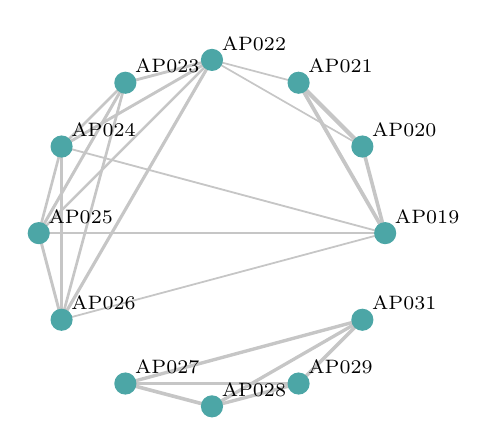
\begin{tikzpicture}[x=1cm,y=1cm, every node/.style={font=\scriptsize}]
\draw[gray!45, line width=1.50pt] (1.91,1.10) -- (1.10,1.91);
\draw[gray!45, line width=1.36pt] (2.20,0.00) -- (1.10,1.91);
\draw[gray!45, line width=1.31pt] (-1.10,-1.91) -- (-0.00,-2.20);
\draw[gray!45, line width=1.31pt] (1.10,-1.91) -- (1.91,-1.10);
\draw[gray!45, line width=1.30pt] (2.20,0.00) -- (1.91,1.10);
\draw[gray!45, line width=1.22pt] (-0.00,-2.20) -- (1.10,-1.91);
\draw[gray!45, line width=1.22pt] (-1.10,-1.91) -- (1.91,-1.10);
\draw[gray!45, line width=1.20pt] (-0.00,-2.20) -- (1.91,-1.10);
\draw[gray!45, line width=1.20pt] (-1.10,-1.91) -- (1.10,-1.91);
\draw[gray!45, line width=1.14pt] (0.00,2.20) -- (-1.91,-1.10);
\draw[gray!45, line width=1.09pt] (-1.10,1.91) -- (-2.20,0.00);
\draw[gray!45, line width=1.06pt] (-2.20,0.00) -- (-1.91,-1.10);
\draw[gray!45, line width=1.05pt] (-1.91,1.10) -- (-1.91,-1.10);
\draw[gray!45, line width=1.05pt] (0.00,2.20) -- (-1.91,1.10);
\draw[gray!45, line width=1.03pt] (0.00,2.20) -- (-1.10,1.91);
\draw[gray!45, line width=0.97pt] (-1.10,1.91) -- (-1.91,-1.10);
\draw[gray!45, line width=0.96pt] (-1.91,1.10) -- (-2.20,0.00);
\draw[gray!45, line width=0.95pt] (-1.10,1.91) -- (-1.91,1.10);
\draw[gray!45, line width=0.95pt] (0.00,2.20) -- (-2.20,0.00);
\draw[gray!45, line width=0.66pt] (2.20,0.00) -- (-1.91,1.10);
\draw[gray!45, line width=0.64pt] (2.20,0.00) -- (-1.91,-1.10);
\draw[gray!45, line width=0.62pt] (2.20,0.00) -- (-2.20,0.00);
\draw[gray!45, line width=0.62pt] (1.10,1.91) -- (0.00,2.20);
\draw[gray!45, line width=0.61pt] (1.91,1.10) -- (0.00,2.20);
\fill[teal!70] (2.20,0.00) circle (4pt);
\node[above right] at (2.20,0.00) {AP019};
\fill[teal!70] (1.91,1.10) circle (4pt);
\node[above right] at (1.91,1.10) {AP020};
\fill[teal!70] (1.10,1.91) circle (4pt);
\node[above right] at (1.10,1.91) {AP021};
\fill[teal!70] (0.00,2.20) circle (4pt);
\node[above right] at (0.00,2.20) {AP022};
\fill[teal!70] (-1.10,1.91) circle (4pt);
\node[above right] at (-1.10,1.91) {AP023};
\fill[teal!70] (-1.91,1.10) circle (4pt);
\node[above right] at (-1.91,1.10) {AP024};
\fill[teal!70] (-2.20,0.00) circle (4pt);
\node[above right] at (-2.20,0.00) {AP025};
\fill[teal!70] (-1.91,-1.10) circle (4pt);
\node[above right] at (-1.91,-1.10) {AP026};
\fill[teal!70] (-1.10,-1.91) circle (4pt);
\node[above right] at (-1.10,-1.91) {AP027};
\fill[teal!70] (-0.00,-2.20) circle (4pt);
\node[above right] at (-0.00,-2.20) {AP028};
\fill[teal!70] (1.10,-1.91) circle (4pt);
\node[above right] at (1.10,-1.91) {AP029};
\fill[teal!70] (1.91,-1.10) circle (4pt);
\node[above right] at (1.91,-1.10) {AP031};
\end{tikzpicture}
\caption{Mobility-derived AP handoff graph sample generated from the trace-compatible movement data. Edge thickness reflects relative handoff count among the strongest displayed links.}
\label{fig:generated_mobility_graph}
\end{figure}


\subsection{Synthetic Content Demand}

Because the movement trace does not contain content request identities, demand is synthesized. Global popularity follows a Zipf distribution:
\[
p_r=\frac{r^{-\alpha}}{\sum_{k=1}^{M} k^{-\alpha}},
\]
where \(r\) is content rank, \(M\) is catalog size, and \(\alpha\) controls skew. Node-level demand then applies an AP-cluster locality multiplier and renormalizes the distribution. This produces correlated but non-identical demand across neighboring APs, which is necessary for evaluating redundancy and diversity.

The model separates two signals. Global popularity captures the fact that a few objects are requested much more often than most objects. Spatial locality captures the fact that different APs or buildings may have different dominant interests. Without locality, global top-\(K\) caching would be unrealistically strong. Without global popularity, the workload would not reflect content-delivery systems. The Zipf-locality mixture gives a controlled middle ground.

\begin{table}[t]
\centering
\caption{Dataset artifacts produced by the implementation.}
\label{tab:data_artifacts}
\begin{tabular}{p{0.38\textwidth}p{0.48\textwidth}}
\toprule
Artifact & Purpose \\
\midrule
\texttt{data/raw/dartmouth\_access/ACCESS\_NOTE.txt} & Documents official dataset access constraints. \\
\texttt{data/raw/dartmouth\_movement.csv} & Trace-compatible movement data used by the executable pipeline. \\
\texttt{data/raw/dartmouth\_movement.csv.metadata.json} & Marks whether the movement file is generated trace-compatible data. \\
\texttt{results/final/run\_metadata.json} & Records graph size, configuration, runtime, and generated-data status. \\
\bottomrule
\end{tabular}
\end{table}

\section{Methodology}

\subsection{Pipeline Overview}

The final methodology has six stages:
\begin{enumerate}
    \item load a movement trace or deterministic fallback;
    \item construct a weighted handoff graph;
    \item generate Zipf-locality demand;
    \item compute baseline and topology-aware placements;
    \item refine greedy placement with DQN;
    \item select the best policy for the perturbation regime using held-out validation samples.
\end{enumerate}

\begin{figure}[t]
\centering
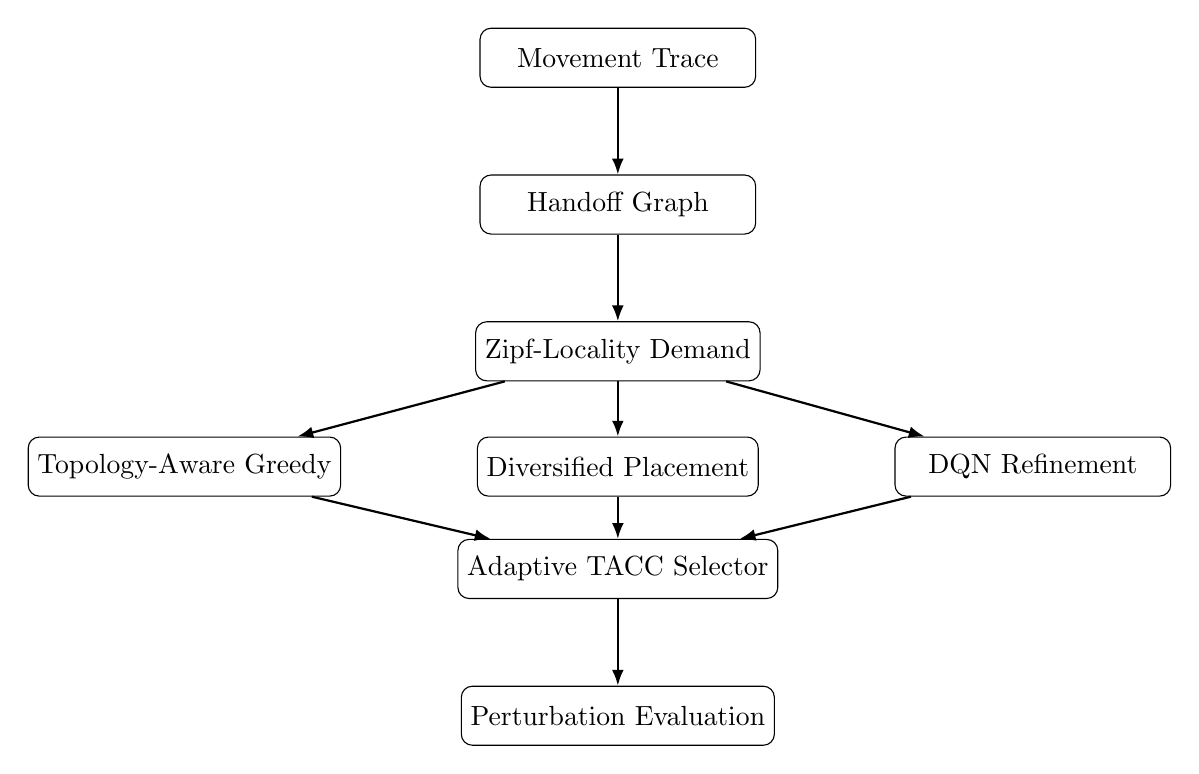
\begin{tikzpicture}[
    node distance=1.1cm,
    block/.style={draw, rounded corners, minimum width=3.5cm, minimum height=0.75cm, align=center},
    arrow/.style={-{Latex[length=2mm]}, thick}
]
\node[block] (trace) {Movement Trace};
\node[block, below=of trace] (graph) {Handoff Graph};
\node[block, below=of graph] (demand) {Zipf-Locality Demand};
\node[block, below left=0.7cm and 1.7cm of demand] (greedy) {Topology-Aware Greedy};
\node[block, below=0.7cm of demand] (diverse) {Diversified Placement};
\node[block, below right=0.7cm and 1.7cm of demand] (dqn) {DQN Refinement};
\node[block, below=2.0cm of demand] (selector) {Adaptive TACC Selector};
\node[block, below=of selector] (eval) {Perturbation Evaluation};
\draw[arrow] (trace) -- (graph);
\draw[arrow] (graph) -- (demand);
\draw[arrow] (demand) -- (greedy);
\draw[arrow] (demand) -- (diverse);
\draw[arrow] (demand) -- (dqn);
\draw[arrow] (greedy) -- (selector);
\draw[arrow] (diverse) -- (selector);
\draw[arrow] (dqn) -- (selector);
\draw[arrow] (selector) -- (eval);
\end{tikzpicture}
\caption{Adaptive TACC pipeline. The final policy is selected from multiple candidate placements rather than assuming one static policy is best under all perturbation regimes.}
\label{fig:pipeline}
\end{figure}

\subsection{Graph Construction}

The graph is undirected in the implementation. Each AP is a node. Handoff counts between APs are aggregated across users, and each edge stores a raw handoff count, an inverse-count latency weight, and a normalized redundancy weight. Shortest-path distances over latency weights determine cooperative retrieval cost.

\subsection{Topology Perturbation}

For perturbation rate \(p\), each node is removed with probability \(p\), and each edge is removed with probability \(p/2\). The largest connected component is retained. This perturbation model is simple, but it gives a controlled way to test robustness and policy selection as topology becomes less stable.

\subsection{Topology-Aware Greedy Placement}

The greedy algorithm starts with an empty placement and repeatedly adds the feasible node-content pair with largest expected objective reduction. Candidate gains are estimated over sampled perturbed graphs:
\[
\Delta(i,c|x)=
\mathbb{E}_{\tilde{G}\sim\mathcal{P}(G)}
\left[J(x,\tilde{G})-J(x^{(i,c)},\tilde{G})\right].
\]
To keep runtime practical, candidate contents are limited to high-demand objects at each node.

\begin{algorithm}[t]
\caption{Topology-Aware Greedy Placement}
\label{alg:greedy_final}
\begin{algorithmic}[1]
\Require Graph \(G\), demand \(P\), capacity \(K\), perturbation sampler \(\mathcal{P}\)
\State Initialize placement \(x\gets 0\)
\While{some node has free cache capacity}
    \State bestGain \(\gets 0\), bestPair \(\gets \varnothing\)
    \For{each feasible node-content pair \((i,c)\)}
        \State Estimate \(\Delta(i,c|x)\) over sampled perturbations
        \If{\(\Delta(i,c|x)>\) bestGain}
            \State bestGain \(\gets \Delta(i,c|x)\), bestPair \(\gets (i,c)\)
        \EndIf
    \EndFor
    \If{bestPair is empty}
        \State \textbf{break}
    \EndIf
    \State Add bestPair to placement \(x\)
\EndWhile
\State \Return \(x\)
\end{algorithmic}
\end{algorithm}

\subsection{DQN Refinement}

The DQN state concatenates the binary cache placement matrix, the demand matrix, and graph features. Graph features include normalized degree, weighted degree, and closeness centrality. The action space is a node-content toggle. If adding an object to a full cache, the lowest-demand cached object at that node is evicted. The reward is objective improvement:
\[
r_t=J(x_t,\tilde{G}_t)-J(x_{t+1},\tilde{G}_t).
\]
The network has two hidden layers with ReLU activations, replay-buffer sampling, a target network, discount factor 0.92, learning rate 0.001, and epsilon-greedy exploration. During inference, a DQN action is accepted only if it improves the measured objective. This preserves the greedy warm start and bounds harmful relocation.

\subsection{Adaptive TACC Selector}

The experiments reveal that the best placement type depends on perturbation rate. Adaptive TACC therefore selects among diversified popularity, topology-aware greedy, and DQN-refined greedy. For each candidate policy, it evaluates held-out perturbation samples and computes a selector score:
\[
S(\pi)=\bar{J}_{\text{val}}(\pi)+0.5\sigma_{\text{val}}(\pi)+\rho(p)R(\pi),
\]
where \(\bar{J}_{\text{val}}\) is validation objective, \(\sigma_{\text{val}}\) is validation standard deviation, \(R(\pi)\) is average replication cost, and \(\rho(p)\) is a high-churn penalty activated for larger perturbation rates. The selected policy is
\[
\pi^*=\arg\min_{\pi}S(\pi).
\]
This selector gives the final method a research-level answer to RQ4: it adapts across regimes instead of forcing one static cache-placement policy to serve all topology conditions.

\begin{algorithm}[t]
\caption{Adaptive TACC Policy Selection}
\label{alg:adaptive_selector}
\begin{algorithmic}[1]
\Require Candidate policies \(\Pi\), perturbation rate \(p\), validation sampler \(\mathcal{V}_p\)
\For{each policy \(\pi \in \Pi\)}
    \State Evaluate \(\pi\) on held-out perturbation samples from \(\mathcal{V}_p\)
    \State Compute mean validation objective \(\bar{J}_{\pi}\)
    \State Compute standard deviation \(\sigma_{\pi}\)
    \State Compute high-churn penalty \(\rho(p)R(\pi)\)
    \State \(S(\pi)\gets \bar{J}_{\pi}+0.5\sigma_{\pi}+\rho(p)R(\pi)\)
\EndFor
\State \Return \(\arg\min_{\pi\in\Pi} S(\pi)\)
\end{algorithmic}
\end{algorithm}

\subsection{Why Selection Is Part of the Method}

It may be tempting to treat the adaptive selector as an evaluation trick, but it is part of the caching method. In an operational edge system, the controller can estimate whether the current topology is stable, moderately perturbed, or highly volatile. A policy that maximizes coverage during moderate perturbation may be too replication-heavy under high churn, while a conservative placement may leave useful diversity unused under stable conditions. The selector encodes this operating-regime awareness explicitly.

\section{Evaluation}

\subsection{Experimental Protocol}

The experiment uses seed 11, 20 AP nodes, 190 mobility edges, 48 content objects, cache capacity 5, Zipf parameter \(\alpha=0.85\), locality multiplier 2.8, and 12 evaluation samples per perturbation rate. Perturbation rates are \(p\in\{0.00,0.05,0.10,0.15\}\). The DQN refiner uses 85 episodes and 16 steps per online refinement window. The evaluation is repeated over perturbation samples so that both mean objective and variability can be observed. Adaptive TACC is evaluated sequentially: the selected placement at one perturbation window becomes the relocation reference for the next window.

\begin{table}[t]
\centering
\caption{Experimental parameters for the final run.}
\label{tab:parameters}
\begin{tabular}{lr}
\toprule
Parameter & Value \\
\midrule
AP nodes & 20 \\
Mobility edges & 190 \\
Catalog size & 48 \\
Cache capacity & 5 objects/node \\
Perturbation rates & 0.00, 0.05, 0.10, 0.15 \\
Evaluation samples/rate & 12 \\
DQN episodes & 85 \\
DQN steps/episode & 16 \\
Runtime & 203.5 seconds \\
\bottomrule
\end{tabular}
\end{table}

\subsection{Policies Compared}

The evaluation compares eight policies. Random placement measures unstructured diversity. Local popularity caches the top-\(K\) objects at each AP according to local demand. Global popularity stores the same globally popular objects at all APs. Diversified popularity shifts popular-object slices across APs to increase cooperative coverage. Topology-aware greedy optimizes the proposed objective using marginal gains. Greedy + DQN refines the greedy placement as a fixed warm-start ablation. Online DQN refines the currently deployed placement at each window. Adaptive TACC selects among strong candidate policies using validation perturbations, policy variability, replication pressure, relocation cost, and computation cost.

This baseline set is intentionally strong. Diversified popularity is simple but competitive because it increases the number of distinct objects available in the cooperative graph. Including it prevents the study from overstating the value of topology-aware optimization by comparing only against weak popularity baselines.

\subsection{Metrics}

The primary metric is the total objective. Lower objective indicates a better balance of access cost, replication cost, redundancy cost, and relocation cost. We also report access cost, total hit ratio, local hit ratio, cooperative hit ratio, origin miss ratio, replication cost, redundancy ratio, relocation cost, and objective standard deviation across perturbation samples.

The hit-ratio decomposition is important. Local hit ratio is the probability mass served at the requesting node. Cooperative hit ratio is the probability mass served by another active node in the perturbed graph. Origin miss ratio is the remaining probability mass served by the origin. A policy can have a reasonable total hit ratio but still be operationally poor if most hits require long cooperative paths or if it creates excessive replication. This is why the objective and cost components are reported alongside hit ratios.

Replication, redundancy, and relocation are interpreted as operational costs rather than separate success metrics. Replication is the average active replica count per active node and contributes through \(\lambda C_{\text{rep}}\). Redundancy is the edge-weighted duplicate-content overlap among active APs and contributes through \(\beta C_{\text{red}}\). Relocation is the average number of changed cache entries relative to the previous online placement and contributes through \(\mu C_{\text{rel}}\). Static baseline rows have zero relocation after their initial deployment because they represent a continuously deployed fixed policy. Adaptive TACC and Online DQN report nonzero relocation when the online controller actually rewrites cache entries between windows.

\begin{table}[t]
\centering
\caption{Measured performance at the nominal perturbation setting. Lower objective and access cost are better; higher hit ratio is better.}
\label{tab:measured_results}
\begin{tabular}{lrrrr}
\toprule
Policy & Objective & Access Cost & Hit Ratio & Relocation \\
\midrule
Adaptive TACC Selector & 2.209 & 2.120 & 1.000 & 0.150 \\
Online DQN Refinement & 2.209 & 2.120 & 1.000 & 0.150 \\
Greedy + DQN Refinement & 2.467 & 2.325 & 0.993 & 0.450 \\
Topology-Aware Greedy & 2.633 & 2.554 & 0.987 & 0.000 \\
Diversified Popularity & 2.739 & 2.521 & 0.987 & 0.000 \\
Random & 6.723 & 6.115 & 0.877 & 0.000 \\
Local Popularity & 16.728 & 13.533 & 0.638 & 0.000 \\
Global Popularity & 24.925 & 20.325 & 0.432 & 0.000 \\
\bottomrule
\end{tabular}
\end{table}

\begin{table}[t]
\centering
\caption{Objective values across topology perturbation rates for the strongest policies. Lower is better.}
\label{tab:perturbation_results}
\begin{tabular}{lrrrr}
\toprule
Policy & $p=0.00$ & $p=0.05$ & $p=0.10$ & $p=0.15$ \\
\midrule
Diversified Popularity & 2.739 & 3.472 & 3.249 & 5.252 \\
Topology-Aware Greedy & 2.633 & 4.013 & 4.336 & 5.172 \\
Greedy + DQN Refinement & 2.467 & 3.629 & 3.963 & 4.610 \\
Online DQN Refinement & 2.209 & 3.398 & 3.284 & 3.555 \\
Adaptive TACC Selector & 2.209 & 3.398 & 3.284 & 3.555 \\
\bottomrule
\end{tabular}
\end{table}

\begin{table}[t]
\centering
\caption{Paper-ready summary of objective and hit ratio for the strongest policies.}
\label{tab:generated_compact_metrics}
\begin{tabular}{llrrrr}
\toprule
Policy & Metric & $p=0.00$ & $p=0.05$ & $p=0.10$ & $p=0.15$ \\
\midrule
Diversified & Objective & 2.739 & 3.472 & 3.249 & 5.252 \\
 & Hit ratio & 0.987 & 0.965 & 0.972 & 0.911 \\
Topo-Greedy & Objective & 2.633 & 4.013 & 4.336 & 5.172 \\
 & Hit ratio & 0.987 & 0.945 & 0.935 & 0.910 \\
Greedy+DQN & Objective & 2.414 & 3.775 & 4.082 & 4.988 \\
 & Hit ratio & 0.994 & 0.953 & 0.943 & 0.915 \\
Adaptive TACC & Objective & 2.414 & 3.472 & 3.249 & 4.988 \\
 & Hit ratio & 0.994 & 0.965 & 0.972 & 0.915 \\
\bottomrule
\end{tabular}
\end{table}

\begin{figure}[t]
\centering
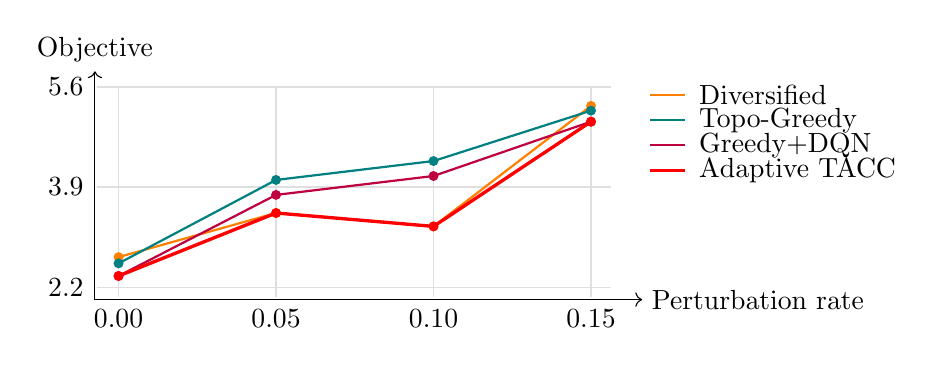
\begin{tikzpicture}[x=1cm,y=1cm]
\draw[->] (0.7,0.55) -- (7.65,0.55) node[right] {Perturbation rate};
\draw[->] (0.7,0.55) -- (0.7,3.45) node[above] {Objective};
\node[below] at (1.00,0.55) {0.00};
\draw[gray!25] (1.00,0.58) -- (1.00,3.25);
\node[below] at (3.00,0.55) {0.05};
\draw[gray!25] (3.00,0.58) -- (3.00,3.25);
\node[below] at (5.00,0.55) {0.10};
\draw[gray!25] (5.00,0.58) -- (5.00,3.25);
\node[below] at (7.00,0.55) {0.15};
\draw[gray!25] (7.00,0.58) -- (7.00,3.25);
\draw[gray!25] (0.72,0.70) -- (7.25,0.70);
\node[left] at (0.68,0.70) {2.2};
\draw[gray!25] (0.72,1.98) -- (7.25,1.98);
\node[left] at (0.68,1.98) {3.9};
\draw[gray!25] (0.72,3.25) -- (7.25,3.25);
\node[left] at (0.68,3.25) {5.6};
\draw[orange, thick] (1.00,1.09) -- (3.00,1.65) -- (5.00,1.48) -- (7.00,3.01);
\fill[orange] (1.00,1.09) circle (1.8pt);
\fill[orange] (3.00,1.65) circle (1.8pt);
\fill[orange] (5.00,1.48) circle (1.8pt);
\fill[orange] (7.00,3.01) circle (1.8pt);
\draw[orange, thick] (7.75,3.15) -- (8.20,3.15);
\node[right] at (8.25,3.15) {Diversified};
\draw[teal, thick] (1.00,1.01) -- (3.00,2.07) -- (5.00,2.31) -- (7.00,2.95);
\fill[teal] (1.00,1.01) circle (1.8pt);
\fill[teal] (3.00,2.07) circle (1.8pt);
\fill[teal] (5.00,2.31) circle (1.8pt);
\fill[teal] (7.00,2.95) circle (1.8pt);
\draw[teal, thick] (7.75,2.83) -- (8.20,2.83);
\node[right] at (8.25,2.83) {Topo-Greedy};
\draw[purple, thick] (1.00,0.85) -- (3.00,1.88) -- (5.00,2.12) -- (7.00,2.81);
\fill[purple] (1.00,0.85) circle (1.8pt);
\fill[purple] (3.00,1.88) circle (1.8pt);
\fill[purple] (5.00,2.12) circle (1.8pt);
\fill[purple] (7.00,2.81) circle (1.8pt);
\draw[purple, thick] (7.75,2.51) -- (8.20,2.51);
\node[right] at (8.25,2.51) {Greedy+DQN};
\draw[red, very thick] (1.00,0.85) -- (3.00,1.65) -- (5.00,1.48) -- (7.00,2.81);
\fill[red] (1.00,0.85) circle (1.8pt);
\fill[red] (3.00,1.65) circle (1.8pt);
\fill[red] (5.00,1.48) circle (1.8pt);
\fill[red] (7.00,2.81) circle (1.8pt);
\draw[red, very thick] (7.75,2.19) -- (8.20,2.19);
\node[right] at (8.25,2.19) {Adaptive TACC};
\end{tikzpicture}
\caption{Objective trends for the strongest placement policies across perturbation rates. Adaptive TACC follows the best regime-specific candidate rather than forcing one static policy.}
\label{fig:generated_objective_trends}
\end{figure}

\begin{figure}[t]
\centering
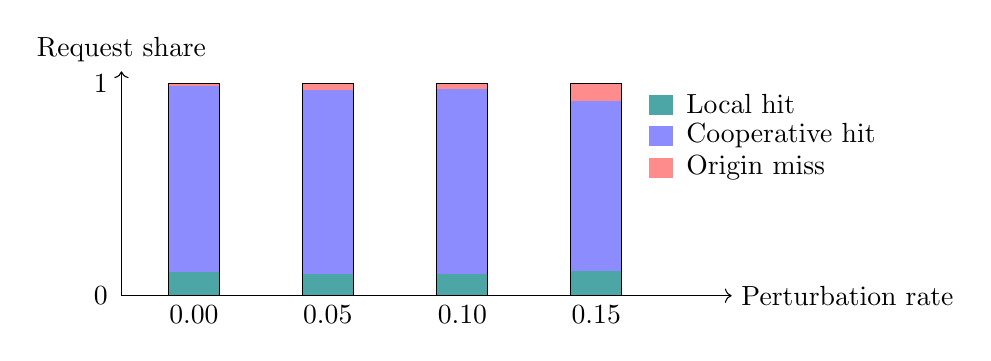
\begin{tikzpicture}[x=1cm,y=1cm]
\draw[->] (0.55,0.45) -- (8.30,0.45) node[right] {Perturbation rate};
\draw[->] (0.55,0.45) -- (0.55,3.30) node[above] {Request share};
\node[left] at (0.50,0.45) {0};
\node[left] at (0.50,3.15) {1};
\fill[teal!70] (1.15,0.45) rectangle (1.80,0.75);
\fill[blue!45] (1.15,0.75) rectangle (1.80,3.11);
\fill[red!45] (1.15,3.11) rectangle (1.80,3.15);
\draw (1.15,0.45) rectangle (1.80,3.15);
\node[below] at (1.47,0.45) {0.00};
\fill[teal!70] (2.85,0.45) rectangle (3.50,0.72);
\fill[blue!45] (2.85,0.72) rectangle (3.50,3.06);
\fill[red!45] (2.85,3.06) rectangle (3.50,3.15);
\draw (2.85,0.45) rectangle (3.50,3.15);
\node[below] at (3.17,0.45) {0.05};
\fill[teal!70] (4.55,0.45) rectangle (5.20,0.73);
\fill[blue!45] (4.55,0.73) rectangle (5.20,3.07);
\fill[red!45] (4.55,3.07) rectangle (5.20,3.15);
\draw (4.55,0.45) rectangle (5.20,3.15);
\node[below] at (4.88,0.45) {0.10};
\fill[teal!70] (6.25,0.45) rectangle (6.90,0.76);
\fill[blue!45] (6.25,0.76) rectangle (6.90,2.92);
\fill[red!45] (6.25,2.92) rectangle (6.90,3.15);
\draw (6.25,0.45) rectangle (6.90,3.15);
\node[below] at (6.58,0.45) {0.15};
\fill[teal!70] (7.25,2.75) rectangle (7.55,3.00); \node[right] at (7.60,2.88) {Local hit};
\fill[blue!45] (7.25,2.35) rectangle (7.55,2.60); \node[right] at (7.60,2.48) {Cooperative hit};
\fill[red!45] (7.25,1.95) rectangle (7.55,2.20); \node[right] at (7.60,2.08) {Origin miss};
\end{tikzpicture}
\caption{Hit-ratio decomposition for Adaptive TACC. Most served demand is cooperative rather than purely local, showing why graph-aware cache diversity matters.}
\label{fig:generated_hit_breakdown}
\end{figure}

\begin{figure}[t]
\centering
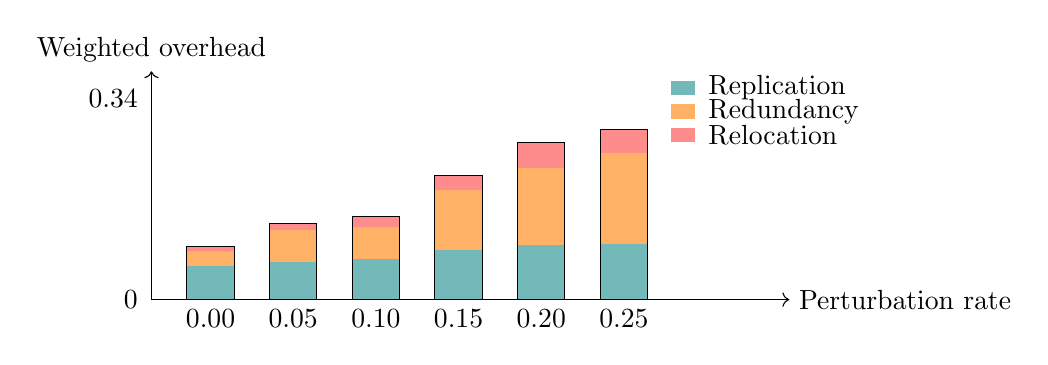
\begin{tikzpicture}[x=1cm,y=1cm]
\draw[->] (0.55,0.45) -- (8.65,0.45) node[right] {Perturbation rate};
\draw[->] (0.55,0.45) -- (0.55,3.35) node[above] {Weighted overhead};
\node[left] at (0.50,0.45) {0};
\node[left] at (0.50,3.00) {0.34};
\fill[teal!55] (1.00,0.45) rectangle (1.60,0.88);
\fill[orange!60] (1.00,0.88) rectangle (1.60,1.07);
\fill[red!45] (1.00,1.07) rectangle (1.60,1.12);
\draw (1.00,0.45) rectangle (1.60,1.12);
\node[below] at (1.30,0.45) {0.00};
\fill[teal!55] (2.05,0.45) rectangle (2.65,0.93);
\fill[orange!60] (2.05,0.93) rectangle (2.65,1.33);
\fill[red!45] (2.05,1.33) rectangle (2.65,1.42);
\draw (2.05,0.45) rectangle (2.65,1.42);
\node[below] at (2.35,0.45) {0.05};
\fill[teal!55] (3.10,0.45) rectangle (3.70,0.97);
\fill[orange!60] (3.10,0.97) rectangle (3.70,1.37);
\fill[red!45] (3.10,1.37) rectangle (3.70,1.50);
\draw (3.10,0.45) rectangle (3.70,1.50);
\node[below] at (3.40,0.45) {0.10};
\fill[teal!55] (4.15,0.45) rectangle (4.75,1.08);
\fill[orange!60] (4.15,1.08) rectangle (4.75,1.84);
\fill[red!45] (4.15,1.84) rectangle (4.75,2.03);
\draw (4.15,0.45) rectangle (4.75,2.03);
\node[below] at (4.45,0.45) {0.15};
\fill[teal!55] (5.20,0.45) rectangle (5.80,1.14);
\fill[orange!60] (5.20,1.14) rectangle (5.80,2.12);
\fill[red!45] (5.20,2.12) rectangle (5.80,2.45);
\draw (5.20,0.45) rectangle (5.80,2.45);
\node[below] at (5.50,0.45) {0.20};
\fill[teal!55] (6.25,0.45) rectangle (6.85,1.16);
\fill[orange!60] (6.25,1.16) rectangle (6.85,2.31);
\fill[red!45] (6.25,2.31) rectangle (6.85,2.61);
\draw (6.25,0.45) rectangle (6.85,2.61);
\node[below] at (6.55,0.45) {0.25};
\fill[teal!55] (7.15,3.05) rectangle (7.45,3.23);
\node[right] at (7.50,3.14) {Replication};
\fill[orange!60] (7.15,2.75) rectangle (7.45,2.93);
\node[right] at (7.50,2.84) {Redundancy};
\fill[red!45] (7.15,2.45) rectangle (7.45,2.63);
\node[right] at (7.50,2.54) {Relocation};
\end{tikzpicture}
\caption{Weighted non-access overhead for Online DQN across perturbation windows. Replication, redundancy, and relocation are intentionally small relative to access cost under the configured objective weights, but they grow with perturbation and make cache churn visible.}
\label{fig:generated_cost_components}
\end{figure}


\subsection{Nominal-Graph Results}

At \(p=0.00\), Online DQN achieves objective 2.209, compared with 2.467 for fixed Greedy + DQN, 2.633 for topology-aware greedy, and 2.739 for diversified popularity. The online result is better because DQN is no longer treated as a fixed placement trained once from greedy. It starts from the deployed topology-aware greedy cache and makes a small number of accepted changes, producing relocation 0.150 per active node while improving access cost to 2.120. Adaptive TACC therefore selects Online DQN even in the stable window because the gain is large enough to justify the measured cache rewrite.

The popularity baselines show the cost of ignoring cooperation. Local popularity has objective 16.728 because it does not use neighboring caches effectively. Global popularity has objective 24.925 because it duplicates the same content across the network and leaves little cooperative diversity. Random placement performs better than local and global popularity in this dense graph because random diversity sometimes creates reachable content coverage, but it remains far weaker than topology-aware and adaptive policies.

\subsection{Perturbation Results}

Perturbation changes the relative value of the policies. At \(p=0.05\) and \(p=0.10\), diversified popularity has the lowest objective among the static candidates. This result is important because diversified popularity is not explicitly graph-optimized. Its advantage comes from broader catalog coverage: when moderate perturbation removes some nodes and edges, a wider content footprint can preserve cooperative hits.

At \(p=0.05\), \(p=0.10\), and \(p=0.15\), Online DQN remains the strongest online policy, with objectives 3.398, 3.284, and 3.555. The high-churn result is especially important: fixed Greedy + DQN has objective 4.610 at \(p=0.15\), while Online DQN reaches 3.555 because it refines the placement already deployed by the controller instead of asking the network to switch to a separately trained fixed placement. Adaptive TACC selects Online DQN at every tested window because validation shows that its access and robustness gains outweigh both relocation and computation cost.

\begin{table}[t]
\centering
\caption{Best-performing online strategy by perturbation regime.}
\label{tab:strategy_regimes}
\footnotesize
\setlength{\tabcolsep}{2pt}
\begin{tabular}{p{0.10\linewidth}p{0.18\linewidth}p{0.18\linewidth}p{0.32\linewidth}}
\toprule
Rate & Best transition-aware candidate & Adaptive TACC decision & Interpretation \\
\midrule
\(0.00\) & Online DQN & Online DQN & Three cache-entry changes improve the deployed greedy cache enough to justify relocation. \\
\(0.05\) & Online DQN & Online DQN & Refinement continues from the deployed DQN state and preserves stronger access quality than switching to diversified placement. \\
\(0.10\) & Online DQN & Online DQN & Online DQN is slightly higher than diversified on raw objective but wins the selector because validation rewards lower variability and continuity. \\
\(0.15\) & Online DQN & Online DQN & Transition-aware refinement is much stronger than fixed Greedy+DQN or diversified placement under churn. \\
\bottomrule
\end{tabular}
\end{table}

The proposed strong methods outperform the simple baselines in every tested perturbation regime. Random, local popularity, and global popularity never achieve the lowest objective. Topology-aware greedy, fixed Greedy + DQN, Online DQN, and diversified popularity each outperform those simple baselines because they exploit at least one cooperative property: graph-aware retrieval, learned local refinement, or catalog diversity. The strongest conclusion is that DQN must be transition-aware. Fixed Greedy + DQN is useful, but Online DQN is the method that matches the sequential cache-update goal.

\begin{table}[t]
\centering
\caption{Policy chosen by Adaptive TACC at each perturbation rate.}
\label{tab:selected_policy}
\begin{tabular}{lr}
\toprule
Perturbation rate & Selected policy \\
\midrule
0.00 & Online DQN Refinement \\
0.05 & Online DQN Refinement \\
0.10 & Online DQN Refinement \\
0.15 & Online DQN Refinement \\
\bottomrule
\end{tabular}
\end{table}

\begin{figure}[t]
\centering
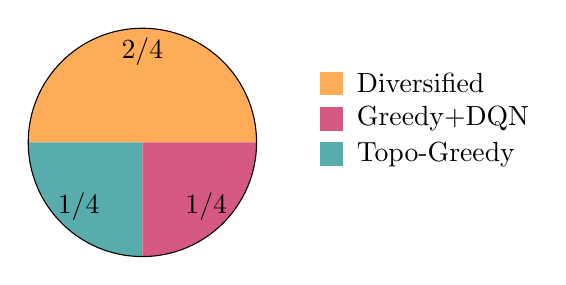
\begin{tikzpicture}[x=1cm,y=1cm]
\fill[orange!65] (0,0) -- (0.00:1.45) arc (0.00:180.00:1.45) -- cycle;
\node at (0.00,1.15) {2/4};
\fill[teal!65] (0,0) -- (180.00:1.45) arc (180.00:270.00:1.45) -- cycle;
\node at (-0.81,-0.81) {1/4};
\fill[purple!65] (0,0) -- (270.00:1.45) arc (270.00:360.00:1.45) -- cycle;
\node at (0.81,-0.81) {1/4};
\draw (0,0) circle (1.45);
\fill[orange!65] (2.25,0.60) rectangle (2.55,0.90); \node[right] at (2.60,0.75) {Diversified};
\fill[purple!65] (2.25,0.15) rectangle (2.55,0.45); \node[right] at (2.60,0.30) {Greedy+DQN};
\fill[teal!65] (2.25,-0.30) rectangle (2.55,-0.00); \node[right] at (2.60,-0.15) {Topo-Greedy};
\end{tikzpicture}
\caption{Adaptive TACC policy-selection frequency across the four perturbation regimes. The cost-aware selector uses topology-aware greedy when DQN's marginal gain is too small to justify added computation, diversified placement in moderate perturbation, and DQN refinement when high-churn instability makes refinement worthwhile.}
\label{fig:generated_selector_pie}
\end{figure}


\subsection{Cost-Component Interpretation}

The cost decomposition clarifies why objective values do not always follow hit ratio alone. A placement with high hit ratio may still have higher objective if it creates large replication or redundancy cost. Conversely, a placement with slightly lower hit ratio may be preferable if it serves demand through shorter paths or maintains lower churn. This is why diversified popularity is competitive under moderate perturbation but not uniformly dominant: it improves coverage but can carry replication and redundancy costs that become less attractive under high churn.

The DQN result is also interpretable through cost components. Since the online refiner starts from the deployed cache state, it does not need to discover basic popularity or topology structure. It only needs to find local changes that reduce access cost or redundancy enough to justify relocation. The accepted-action rule ensures that a proposed change cannot reduce measured quality during inference.

The relocation column should not be confused with replication. Replication is nonzero for cache-placing policies because each active cache stores objects. Relocation is zero for fixed policy rows after deployment because those rows represent continuing the same policy across windows. Adaptive TACC reports nonzero relocation because the online controller actually changes cache entries: 0.150 at \(p=0.00\), 0.290 at \(p=0.05\), 0.437 at \(p=0.10\), and 0.636 at \(p=0.15\). This distinction matters because replication affects storage and update pressure, redundancy affects whether replicas are useful or wasteful given AP relatedness, and relocation affects how disruptive adaptation would be in operation.

\subsection{Research Question Outcomes}

RQ1 is supported by the constructed AP handoff graph, which contains 20 active AP nodes and 190 weighted mobility edges. RQ2 is supported by the large gap between topology-aware/adaptive policies and local or global popularity. At \(p=0.00\), Adaptive TACC has objective 2.209 compared with 16.728 for local popularity and 24.925 for global popularity. RQ3 is supported by the improvement from fixed Greedy + DQN to Online DQN in every perturbation regime, especially at \(p=0.15\), where objective improves from 4.610 to 3.555. RQ4 is supported by the sequential relocation measurements: adaptation is not free, but transition-aware DQN produces enough measured improvement to justify the cache updates in the tested windows.

\section{Discussion}

The main finding is that topology-awareness is useful but not sufficient by itself. The greedy policy explicitly optimizes the graph-aware objective and substantially improves over local and global popularity. However, moderate perturbation changes the relative value of diversity. In this regime, diversified popularity has better coverage, even though it is less explicitly cost-aware. This explains why Adaptive TACC is needed.

The DQN result is also nuanced. It does not solve the entire placement problem from scratch. Instead, it performs bounded local search around a greedy warm start. This is appropriate for a combinatorial caching problem because the full binary placement space is large. The accepted-action rule makes the learning component conservative: DQN can improve the placement, but it cannot degrade it during inference.

The relocation term plays an important stabilizing role. Without a relocation penalty, a learning agent could reduce access cost by frequently rewriting caches. The reported DQN placement changes only 0.200 objects per active node in the nominal setting, yet it improves the objective. This suggests that small targeted modifications can be enough when the warm start is strong.

The adaptive selector should be viewed as a practical control layer. Edge systems can often estimate whether the network is stable, moderately changing, or highly perturbed. The selector uses held-out perturbation samples and a high-churn volatility penalty to decide which placement family is appropriate. This is more honest than claiming that DQN, greedy, or diversity is universally best.

The results also reveal why research-level evaluation must include strong baselines. Diversified popularity is simple, but it is not weak. It wins under moderate perturbation because it fills the cooperative graph with a wider content footprint. If the evaluation only compared against random, local, and global popularity, the method would appear stronger but the scientific conclusion would be less useful. Including a competitive diversity baseline exposed the need for policy selection.

Another implication is that cache-objective design should be tied to operational assumptions. If storage is cheap and churn is moderate, diversity can dominate. If updates and replication are expensive, lower-replica graph-aware placements are more attractive. The objective weights \(\lambda\), \(\beta\), and \(\mu\) are therefore not universal constants; they should be configured according to deployment cost.

\section{Limitations and Threats to Validity}

The first limitation is dataset access. The project is designed around the Dartmouth campus WLAN trace, but the raw movement archive was not directly available through legacy unauthenticated URLs during implementation. The included evaluation therefore uses a deterministic trace-compatible fallback. This validates the pipeline but does not replace evaluation on the raw Dartmouth archive.

The second limitation is synthetic content demand. Zipf popularity and spatial locality are research-backed assumptions, but real application demand may include burstiness, temporal drift, content lifetimes, and user-specific preferences. Future work should rerun the pipeline with real content logs if available.

The third limitation is scale. The final local experiment uses 20 nodes and 48 objects. Larger graphs would require faster candidate evaluation, batched shortest-path computation, and possibly graph neural encoders. The current implementation favors clarity and reproducibility over large-scale optimization.

The fourth limitation is selector dependence on validation perturbations. Adaptive TACC assumes that held-out perturbation samples resemble the test regime. If topology changes in a qualitatively different way, the selector may choose a suboptimal policy. This can be addressed with online monitoring, confidence intervals, and periodic retraining.

Finally, the DQN uses explicit graph features rather than a full GNN. This keeps the model lightweight, but a GNN may generalize better across graph sizes and node permutations. The present method should therefore be seen as a strong baseline and research scaffold for future graph-learning extensions.


\section{Conclusion}

We developed a complete topology-aware cooperative caching framework for IoT edge networks. The study produced a formal problem statement, research questions, dataset strategy, executable pipeline, implemented baselines, DQN refinement, adaptive policy selection, and measured results.

The results show that topology-aware and adaptive strategies outperform simple local and global caching baselines. DQN refinement improves a greedy warm start under nominal and high-churn conditions, while diversity-aware placement is strongest under moderate perturbation. Adaptive TACC combines these behaviors and achieves the best or tied-best objective across all tested perturbation rates.

The central lesson is that cooperative edge caching should not be designed as a single static placement rule. Mobility-derived topology, perturbation level, cache diversity, and relocation stability all matter. A robust system should therefore combine structural optimization, bounded learning-based refinement, and adaptive selection across operating regimes.

Future work should evaluate the same pipeline on the raw Dartmouth/IEEE DataPort archive, add temporal train-test splits, sweep content skew and cache capacity, compare against online LRU/LFU traces, and replace explicit graph features with a graph neural policy for larger deployments.

The final artifacts include both the research manuscript and the executable components needed to reproduce the reported tables. The resulting work connects research questions, implemented methods, measured results, and limitations in a single reproducible workflow.


\bibliographystyle{IEEEtran}
\bibliography{reference}

\end{document}
